\documentclass[a4paper]{article}

%% Language and font encodings
\usepackage[english]{babel}
\usepackage[utf8x]{inputenc}
\usepackage[T1]{fontenc}

%% Sets page size and margins
\usepackage[a4paper,top=3cm,bottom=2cm,left=3cm,right=3cm,marginparwidth=1.75cm]{geometry}

%% Useful packages
\usepackage{amsmath}
\usepackage{graphicx}
\usepackage[colorinlistoftodos]{todonotes}
\usepackage[colorlinks=true, allcolors=blue]{hyperref}
\usepackage{float}
\usepackage{algorithm}
\usepackage[noend]{algpseudocode}
\usepackage{listings}

\graphicspath{ {images/} }

\title{Peg Solitaire Backtracking Assignment}
% \author{}
% Update supervisor and other title stuff in title/title.tex

\begin{document}
\begin{titlepage}

\newcommand{\HRule}{\rule{\linewidth}{0.5mm}} % Defines a new command for the horizontal lines, change thickness here

\center % Center everything on the page
 
%----------------------------------------------------------------------------------------
%	HEADING SECTIONS
%----------------------------------------------------------------------------------------

\textsc{\LARGE University of the Witwatersrand}\\[1.5cm] % Name of your university/college
\textsc{\Large COMS3005: Advanced Analysis of Algorithms}\\[0.5cm] % Major heading such as course name
% \textsc{\large Minor Heading}\\[0.5cm] % Minor heading such as course title

%----------------------------------------------------------------------------------------
%	TITLE SECTION
%----------------------------------------------------------------------------------------
\makeatletter
\HRule \\[0.4cm]
{ \huge \bfseries \@title}\\[0.4cm] % Title of your document
\HRule \\[1.5cm]
 
%----------------------------------------------------------------------------------------
%	AUTHOR SECTION
%----------------------------------------------------------------------------------------
{\large \today}\\[2cm] % Date, change the \today to a set date if you want to be precise

\begin{minipage}{1\textwidth}
  \Large \emph By Bancroft, E. (879192)\\
  \Large \emph And Chalom, J. (711985)\\
\end{minipage}

% If you don't want a supervisor, uncomment the two lines below and remove the section above
%\Large \emph{Author:}\\
%John \textsc{Smith}\\[3cm] % Your name

%----------------------------------------------------------------------------------------
%	DATE SECTION
%----------------------------------------------------------------------------------------



%----------------------------------------------------------------------------------------
%	LOGO SECTION
%----------------------------------------------------------------------------------------

% \includegraphics[width=8cm]{title/logo.png}\\[1cm] % Include a department/university logo - this will require the graphicx package
 
%----------------------------------------------------------------------------------------

\vfill % Fill the rest of the page with whitespace

\end{titlepage}

% \lfoot{School of Computer Science and Applied Mathematics}
\clearpage
\setcounter{page}{1}
% \setcounter{section}{1}
\pagenumbering{arabic}

% \section*{Abstract}


\section{Introduction}
The purpose of the assignment is to implement and analyse a version of the Peg Solitaire game and the backtracking algorithm (to play the game to completion and return a valid path).

\section{Background}
Peg Solitaire is a board game which has a number of holes that can be filled with pegs. We have chosen to use the European/French style of board which has four extra positions for pegs on the board \ref{board}. In this style most of a grid of 49 has peg holes excluding three per corner resulting in 37 peg holes. The aim of the game is to remove pegs until only one peg remains. This is the position one row directly above the central peg, a row above that and the left most peg in the top row. Moves are made when pegs jump over a peg and are placed in an open position. Then a peg which has been jumped over, is then removed. This move can happen in both horizontal and vertical directions. In the European variant, the game has three possible optimal terminal states. Its is possible to hit sub-optimal states where there are more pegs left on the board but no possible moves left \cite{harder}. 

% Have example moves and suboptimal states?
\begin{figure}[H]
	\centering
	\label{board}
	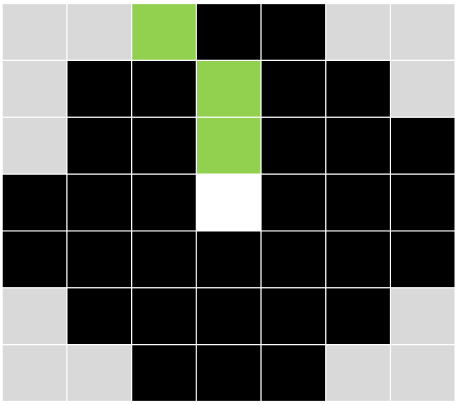
\includegraphics[width=.50\textwidth,scale=.50]{images/board}
	\caption{Diagram of an European Peg Solitaire Board Where the
				Black Squares Represent Peg Positions,
				Green Are Terminal Positions,
				Grey Are Not Positions and
				White is the Central Pixel.
			}
\end{figure}

% cite the wayback machine??
\noindent The backtracking algorithm is similar to a brute force approach to finding solutions to problems but is more systematic. It attempts to follow a logical series of decisions in solving these problems and when a block state occurs the algorithm will backtrack to previous decisions and choose different paths until a terminal (complete) state is reached. The full set of solutions to a problem can be found by continuing to run the algorithm until all paths have been searched but that is not always necessary.

\begin{algorithm}[H]
	\begin{algorithmic}[1]
		\Procedure{FindSolution}{\texttt{start, final, path}}
			\If {\texttt{start.numPegs <= final.numPegs}}
				\State \Return (start = final)
			\Else 
				\For{\texttt{each jump $J \in$ [0,n) x [0,m) x \{NORTH,EAST,SOUTH,WEST\}}}
			        \If {$J$ is a legal jump for start}
			        	\State \texttt{start.makeMove($J$)}
			        	\State \texttt{path.push($J$)}
			        	\State \texttt{found = FindSolution(start, final, path)}

			        	\If {found}
			        		\State \Return {TRUE}
			        	\Else
			        		\State \texttt{start.makeReverseMove($J$)}
			        		\State \texttt{path.pop()}
			        	\EndIf
					\EndIf
		      	\EndFor
		      	\State \Return{FALSE}
			\EndIf 
		\EndProcedure
	\end{algorithmic}
	\caption{Recursive Algorithm (From References \cite{lab5})}\label{euclid}
\end{algorithm}


\subsection{Stack Based Algorithm}
The stack based algorithm we used is adapted from the recursive version. The purpose of implementing the stack based algorithm was to compare it's effciency to that of the recursive based algorithm. Also the recursive algorithm was expected to be much slower.

\begin{algorithm}[H]
	\begin{algorithmic}[1]
		\Procedure{FindSolution}{\texttt{start, outPath, totalNumPegs, numValidMoves}}
			\State currentState $\leftarrow$ start
			\State path $\leftarrow$ start.getMoves()
			\State numPegs $\leftarrow$ currentState.getNumPegs()
			\State found $\leftarrow$ FALSE
			\State i $\leftarrow$ 1

			\State stackVector.push(path)
			\State boardVector.push(currentState)

			\While {found is FALSE and i <= numPegs and stackVector.size() > 0 and path.size() > 0}
				\State path $\leftarrow$ stackVector.pop()
				\State currentState $\leftarrow$ boardVector.pop()

				\While {\texttt{currentState.checkGameEnd() != FALSE}}
					\State numPegs $\leftarrow$ currentState.getNumPegs()
					\State move $\leftarrow$ path.pop()

					\If {\texttt{currentState.checkIfMoveValid(move) == TRUE}}
						\State stackVector.push(path)
						\State boardVector.push(currentState)
						\State numValidMoves = numValidMoves + 1
						\State currentState.makeMove(move)
						\State outPath.push(move)
						\State path $\leftarrow$ currentState.getMoves()
						\State numPegs $\leftarrow$ currentState.getNumPegs()
					\EndIf
				\EndWhile
				\State numPegs $\leftarrow$ currentState.getNumPegs()
				%\If {numPegs == 1}
				\If {currentState.checkGameWin() == TRUE}
					\State found = TRUE
				\Else
					\State found = FALSE
				\EndIf
				%\EndIf
			\EndWhile
			\Return currentState
		\EndProcedure
	\end{algorithmic}
	\caption{Stack Based Algorithm (Adapted From References \cite{lab5})}\label{euclid}
\end{algorithm}

\section{Implementation}
% Comment: Talk about OpenMP, Assumptions any special things ...
% What data structures we used
% Commandline options
% how to build
% how we genereated random states rather than use a database etc...
% what random generator
% terminating conditions
% etc...
% French board
% Average Number of Avilable Peg Moves = Cumulative Num of valid moves / Cumulative Number of Pegs (Across all states)

\subsection{Technology Used}
We made use of c++ 11, its standard libraries and OpenMP to time our results. Our results are saved as comma seperated value files which are then processed and graphed by libre office.\\
To create the stacks in the stack implemntation we used vectors.\\
To generate the pseudorandom numbers we used the Mersenne Twister engine that comes included in the c++ "random" library.\\
%TODO make a refrence to Mersenne  twister. either its wiki page or a mt distrubiton example on cpprefrence
%and this
\subsection{How To Compile and Run}
In order to compile and run the code:\\
% TODO proper styling
Go to root folder of the project and run make.\\
Then run ./bin/game.out to run the game.
\\\\
\noindent Commandline Parameters:
\begin{lstlisting}
	
	Usage Example: ./bin/game.out -rb
	Random state: ./bin/game.out -rr
	Full state: ./bin/game.out -rf
	Run Stacked Based Backtracking: -rb
	Run Recursive Backtracking: -recurse
	Manual: -m
	Help: -h
\end{lstlisting}
% have two tests one for recursive and one for stack
% must show states

\subsection{Our Termination Conditions}
Although both algorithms terminate under similar theoretical conditions (no more moves possible or it has reached a "win" state), due to their different implemntations, the teminating conditions are diffrent.
\subsubsection{Recursive Implementation}
This implentation works very similar to a Depth First Search and will terminate under very similar conditions to a DFS algoritm.\\
These conditions are : 
\begin{itemize}
\item Found one of the three "win" states.
\item Cannot backtrack any further: So the algorithm has returned to the root layer, and as such hasn't found any of the "win" states, and wishes to try backtrack further, however there are no more layers to backtrack too and as such the algorithm will conclude that a "win"  state cannot be found given the current start state and will terminate.
\end{itemize}
\subsubsection{Stack Implementation}
This implementation works diffrently from the recursive as it uses a stack of paths to store the progress down a branch of a tree and create backtrack points when ever the algorithm does a move.\\
The conditions where the stack implemntation will terminate are :
\begin{itemize}
\item Found one of the three "win" states.
\item If the algorithm finds it's self on the orginal path that was generated and the path size of that path is zero (poped off all moves) . i.e. There is nowhere higher to back track too, and all moves on the current path have been exasusted then the algorithm has tried all possible moves and will conclude that a "win"  state cannot be found given the current start state and will terminate.
\end{itemize}
\subsection{Best Case}
We decided that it would be helpfull to have best case data points for both recursive and the stack implemntation to compare with. These best case game states always incude a single path that will result in finding a "win" state.\\
However there is a major issue that we ran into regarding the best case state generator. It only worked up to 17 pegs. This due to the way we generate the backwards path. i.e it will start at a "win" state and try a up reversal, if it can't, it will try a right move reversal,if it can't, then try a down reversal and if that fails try a left move reversal.\\
Contiueing this pattern the board will be filled with n pegs if n<=17. When we try creating 18+ points it will fail to find any valid reverse move and as such 17 points is the maximum number of points we could create with this algorithm.


\subsection{Problems We Encountered}
% Why - recursive due to it relying on heap ... slow internally
% stack is much more efficient use of memory
% We then checked results manually and with tests to ensure the correct choices were made - printed out states
One of the most notable feature/Problem we encountered was that the stack implemntation was incrediably fast relative to the recursive implemntation. Both returned the correct output but because of the recursive implemntation relying on a heap, we only managed to get 17 data points in 30 hours of the program running. \\
The stack implemntation doesn't use the heap (which the recursive alogrithm does), which is internally slow, so therefore allowing the stack implemntation's effciency to far surpass that of the recursive's.\\
The vector stack in c++ also is a much more effcient use of memory compared to storing objects on a heap.\\\

\subsection{Experimental Setup}
% Describe how we test
% Our loops 
% recursive has 3 final states so its run 3 times because its finding 3 different win states
For our experiment we tested with an increasing number of pegs being place randomly throughout the board.\\
Each test will try to find one of the three "win" states based on the  starting state that was generated. This proccess will be timed and the time, together with the number of pegs that were generated will be recoreded.\\
Although with the recursive implemntation we have  to run the same state three times (once for each of the three possible "win" states) the time that is being recorded is the amount of time that it takes to run the instance of the algoritm that finds a  "win" state, or the time it takes for one instance to explore the entire tree, not all three.\\
%TODO explain this better.


\section{Theoretical Analysis}
We assume that our basic opertion used for analysis in the backtracking algorithm for peg-solitaire is generating a new state which is playing a valid move or jumping a peg into a valid empty space (and removing a peg between them). Determining if there are no more moves, and also getting every valid move for a peg are both assumed to take constant time, which is the speed of each conditional by the number of board elements i.e. 49 elements.\\\

\noindent The best case complexity of backtracking for peg-solitaire would be the case where only one path needs to be generated for any number of pegs i.e. no backtracks occur because a game win is found at the end of the first path. In this case the complexity is the number of pegs left on the board or the length of the found path. If we assume this number is represented by the variable n, then the best case complexity is $O(n)$.\\\

% number of moves = 4
% number of pegs
% decreasing number of pegs

\noindent In the worst case complexity event no game win is possible so every possible path has to be traversed by the algorithm. Each peg has the potential to move in four directions but that is unlikely. From our observations of the game being played out moves on a board from a start state tends to allow on average two possible moves per peg when moves are available. This means that on average (based on our observations) the game has a branching factor of 2. Since each path can be considered to be a branch on a tree data structure and the number of branches is the number of pegs which is assumed to be n. This means that the total search space (game-space) size is $2^n$ and so the worst case complexity is directly propotional to this number i.e. the worst case complexity is $O(2^n)$. 

\section{Results}

\section{Empirical Analysis}


\section{Conclusion}
% Talk about comman non-unique states and using hashing and dynamic programming to improve perforamnce

\section{Group Member Contribution}
\begin{table}[H]
\centering
\label{contribution}
\begin{tabular}{|l|l|l|}
\hline
\textbf{Member}         & \textbf{Evan Bancroft 879192} & \textbf{Jason Chalom 711985} \\ \hline
Game                    & 75\%                          & 25\%                         \\ \hline
Back Tracking Algorithm & 50\%                          & 50\%                         \\ \hline
% Complexity Analysis     & \%                          & \%                         \\ \hline
Report                  & 25\%                          & 75\%                         \\ \hline
\end{tabular}
\caption{Contributions of Group Members By Task}
\end{table}

\section*{Acknowledgements}
All drawn diagrams were drawn using \url{http://draw.io/} and charts were made with Libre Office.\\ 
All the programming was done in c++ using OpenMP for its timing functions.\\


\bibliographystyle{plain}
\bibliography{biblio}{}

\end{document}